\documentclass{article}
\usepackage[utf8]{inputenc}
\usepackage{hyperref}
\usepackage{amsmath}

\title{Epidemic Timeseries - Thesis}
\author{Matthew So}
\date{October 2020}
\usepackage{graphicx}
\begin{document}

\maketitle

\tableofcontents


\section{Relevant resources}

\begin{itemize}
    \item \hyperlink{https://docs.google.com/document/d/105QZAGMzl7m6JZiXGLuycXWrZcsydqJ_/edit}{Meeting planner} 
    \item \hyperlink{https://github.com/Apeirogons/COVID-math-thesis}{Overall thesis GitHub repo}
    \item \hyperlink{https://github.com/Apeirogons/COVID-math-thesis/tree/master/shifts}{Shifts folder}
    \item \hyperlink{https://github.com/Apeirogons/COVID-math-thesis/tree/master/epidemic_timeseries}{Folder for phase-plane analysis, mobility PCA, and clustering}    
\end{itemize}


\section{Writeup Todo}
\begin{itemize}
    \item Add relevant images. Particularly important as this project benefits quite a bit from graphics
    
\end{itemize}

\section{Mobility PCA}
\subsection{Explanation of mobility PCA}
Google Mobility data contains detailed daily mobility data for each country. We wanted to use this data to make a single mobility index that was applicable to all countries.

\subsection{Current approach}

Google Mobility tracks mobility in terms of a percent change from baseline in retail and recreation (RR), grocery and pharmacy (G), transit stations (T), workplaces (W), residential (R), and parks (P).

Mobility data for all listed metrics except P smoothed with a 7-day window (one reason was to remove weekend effects; note that performing no smoothing has similar results). Data was taken for all countries with $\geq$ 200 datapoints and naively accumulated. Then, the PCA algorithm from \href{https://scikit-learn.org/stable/}{scikit-learn} was fitted to this data. 

The explained variance of principal component (PC) 1 is 0.894, and the explained variance of PC 2 is 0.041. The components of PC 1 were (last run): RR 0.57781228  G 0.40459858 T 0.53877504  W 0.41191798 R -0.20610189, and the components of PC 2 are: RR 0.26836183  G 0.66819787 T -0.35537018 W -0.59375593 P -0.05156992.

\begin{figure}[h!]
    \centering
    \includegraphics[scale=0.4]{figures/United_States.png}
    \caption{A PCA reconstruction (grey lines) of mobility data for United States.}
    \label{fig:my_label}
\end{figure}


\subsection{Concerns}
No major concerns at this moment. 

Just for documentation purposes: In the past, MS had concerns about a seemingly poor reconstruction accuracy in the latter half of the pandemic. After actually plotting the inverse-transformed PCA-transformed data, I no longer believe this is an issue.


\section{Clustering}
\subsection{Explanation of clustering}
Epidemic timeseries (such as incidence, cumulative case, etc.) curves are qualitatively different. For example, the U.S. incidence timeseries is obviously different from the Canadian incidence timeseries. I would like to algorithmically cluster "similar" timeseries, and hopefully this will give some deeper insight about pandemic responses in different countries. 

\subsection{Current approach}
I intend on trying out several different timeseries distance metrics to determine the pairwise distances between each timeseries. I've currently tried the discrete time warping-Euclidian distance, but other metrics have been \href{https://link.springer.com/chapter/10.1007/978-3-030-28665-1_31}{reported}. In terms of the actual clustering, I need to use an algorithm that can cluster points based on pairwise distance. From some of my experimentation, I thought the DBSCAN algorithm gave some good results. This algorithm seeds a new cluster if it has at least $n$ points that are within $\epsilon$ units from it. Then, if another point is within $\epsilon$ units from a cluster point, it is added to a cluster. If two clusters share a point, they are merged into a single cluster. I define the start of the pandemic as the first point in time at which there are $\geq$ 1 cumulative cases in a country, although I'm not sure of how much this matters (due to the use of DTW)

\begin{figure}[h!]
    \centering
    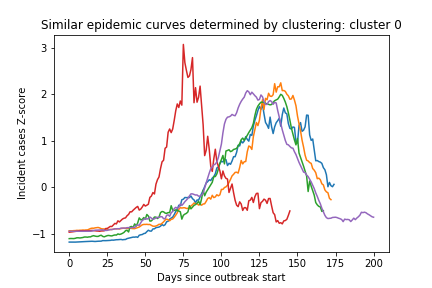
\includegraphics[scale=0.4]{figures/cluster 0.png}
    \includegraphics[scale=0.4]{figures/cluster 3.png}
    \caption{Similar incidence timeseries determined by clustering.}
    \label{fig:my_label}
\end{figure}

\subsection{Concerns}
I don't understand DTW yet. 

\section{Phase-planes and other plots}
\subsection{Explanation of plots}
(For myself): Phase-planes plot two variables that are connected in time against each other. They're sort of similar to the vector field plots that pop up if you search up 'phase plane' in that it shows the evolution of two functions of an underlying variable.

\begin{figure}
    \centering
    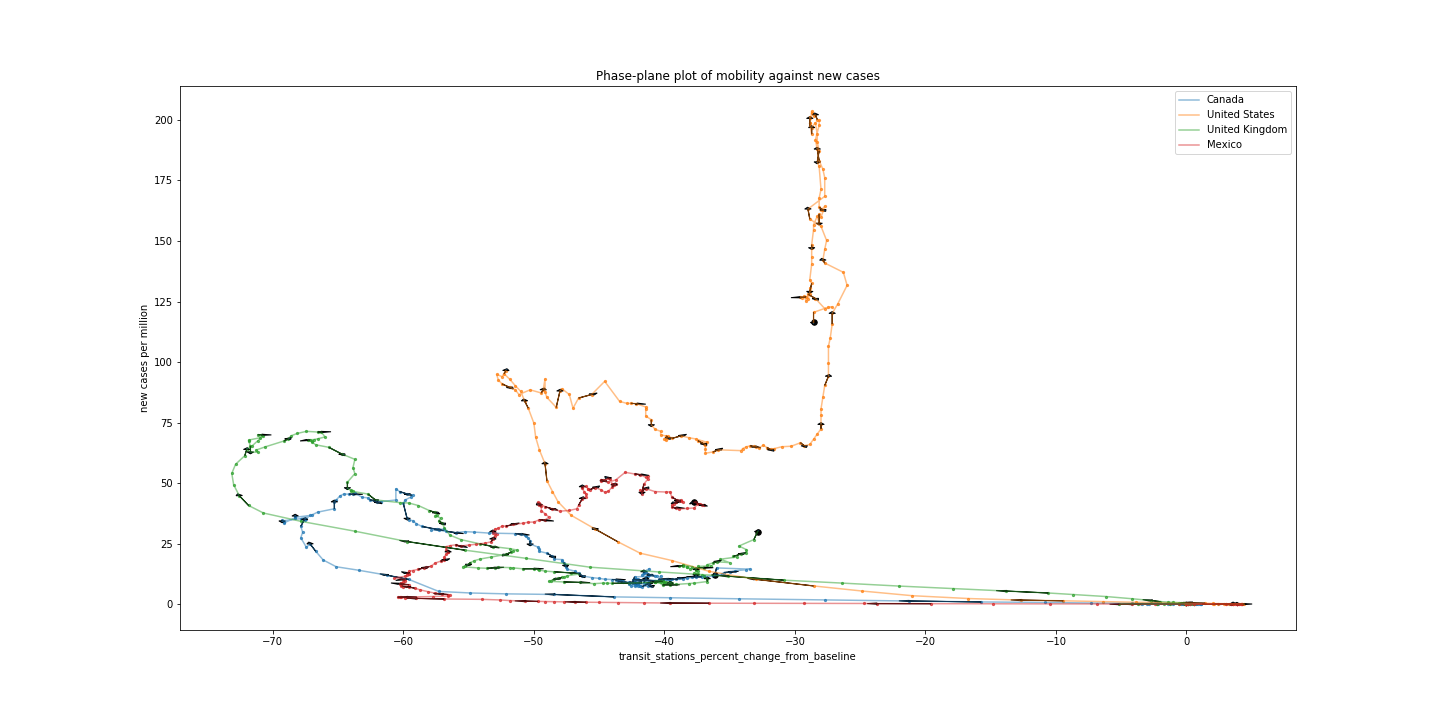
\includegraphics[scale=0.25]{figures/mobility_vs_new_cases.png}
    \caption{A phase plane of transit mobility against new cases for selected countries}
    \label{fig:my_label}
\end{figure}



\subsection{Current approach}
I scatter-plot the two variables under consideration, then connect each dot with lines and add arrows showing the direction of the motion. I also make heavier dots at the end of each phase plane. The plots should be cleaned up a bit (for example, it may be worthwhile to smooth incidence curves).

\subsection{Concerns}
JD is colorblind, so MS should use a colorblind palette.


\section{Shifts}
\subsection{Explanation of shifts}
An exploration of JD's idea found  \href{http://dushoff.github.io/notebook/shifts.html}{here}. The idea is to investigate using the methods of Cori and Wallinga to estimate R(t). We will use deconvolution (currently Richardson-Lucy as used in the \href{https://www.medrxiv.org/content/10.1101/2020.06.18.20134858v3}{Gostic paper}) to provide an estimate of the true incidence curve from the number of new symptomatic infections. 

\subsection{Current approach}
I use code from the \href{https://github.com/cobeylab/Rt_estimation}{Gostic paper} to perform Richardson-Lucy deconvolution in R. I use the \href{https://cran.r-project.org/web/packages/EpiEstim/index.html}{EpiEstim} library to generate R(t) estimates using the Cori and Wallinga-Tenuis methods. 

Like the Gostic paper, I've used a vanilla SEIR model (We need to be able to replicate the results first).

\begin{align}
\frac{dS}{dt} &= -\beta(t) \frac{S}{N}  I \\ 
\frac{dE}{dt} &= \beta(t) \frac{S}{N} I - \gamma E \\
\frac{dI}{dt} &= \gamma E - \mu I \\ 
\frac{dR}{dt} &= \mu I  
\end{align}

Therefore, these are equations representing the \href{https://www.ncbi.nlm.nih.gov/pmc/articles/PMC3935673/}{instantaneous reproductive number}:

\begin{align}
    R_0 = \beta(t)/\mu \\
    R(t) = \beta(t)/\mu \cdot S/N
\end{align}

This is how (I think) you can obtain the generation interval distribution analytically. I may be totally wrong, please help here. It is an addition of exponential distributions of $E \xrightarrow{}I$ and $I \xrightarrow{} R$, exploiting the fact that both the means and variances add up, as well as that two exponential distributions multiplied by each other make a Gamma distribution. It also may not be super necessary now.


$G$: generation interval distribution \\ 
$k$: shape parameter of Gamma distribution\\
$\theta$: scale parameter of Gamma distribution\\

\begin{align}
    Mean(E \xrightarrow{}I) = 1/\gamma \\ 
    Mean(I \xrightarrow{}R) = 1/\mu \\ 
    Var(E \xrightarrow{}I) = 1/\gamma^2 \\ 
    Var(I \xrightarrow{}R) = 1/\mu^2 \\
    Mean(G) = 1/\gamma + 1/\mu = k\theta\\ 
    Var(G) = 1/\gamma^2 + 1/\mu^2 = k\theta^2 \\ 
    k =  Mean(\text{G})^2/Var(\text{G}) \\
    \theta = Var(\text{G})/Mean(\text{G})
\end{align}

This equation represents the cohort reproductive number, which will be estimated with the Wallinga method.

\begin{equation}
    R_{case}(t) = R(t) * G
\end{equation}

\subsection{Progress}
From preliminary testing, the deconvolution method fits the true incidence quite well. However, further testing is required (changing Rt, stochastic effects) to see if it might work well in practice.

The Cori method to the deconvoluted incidence also seems to work well with the static $\beta$ and slowly changing R(t). The Wallinga-Tenuis method seems to fit the slowly changing cohort R(t), but is incredibly slow.

\begin{figure}[h!]
    \centering
    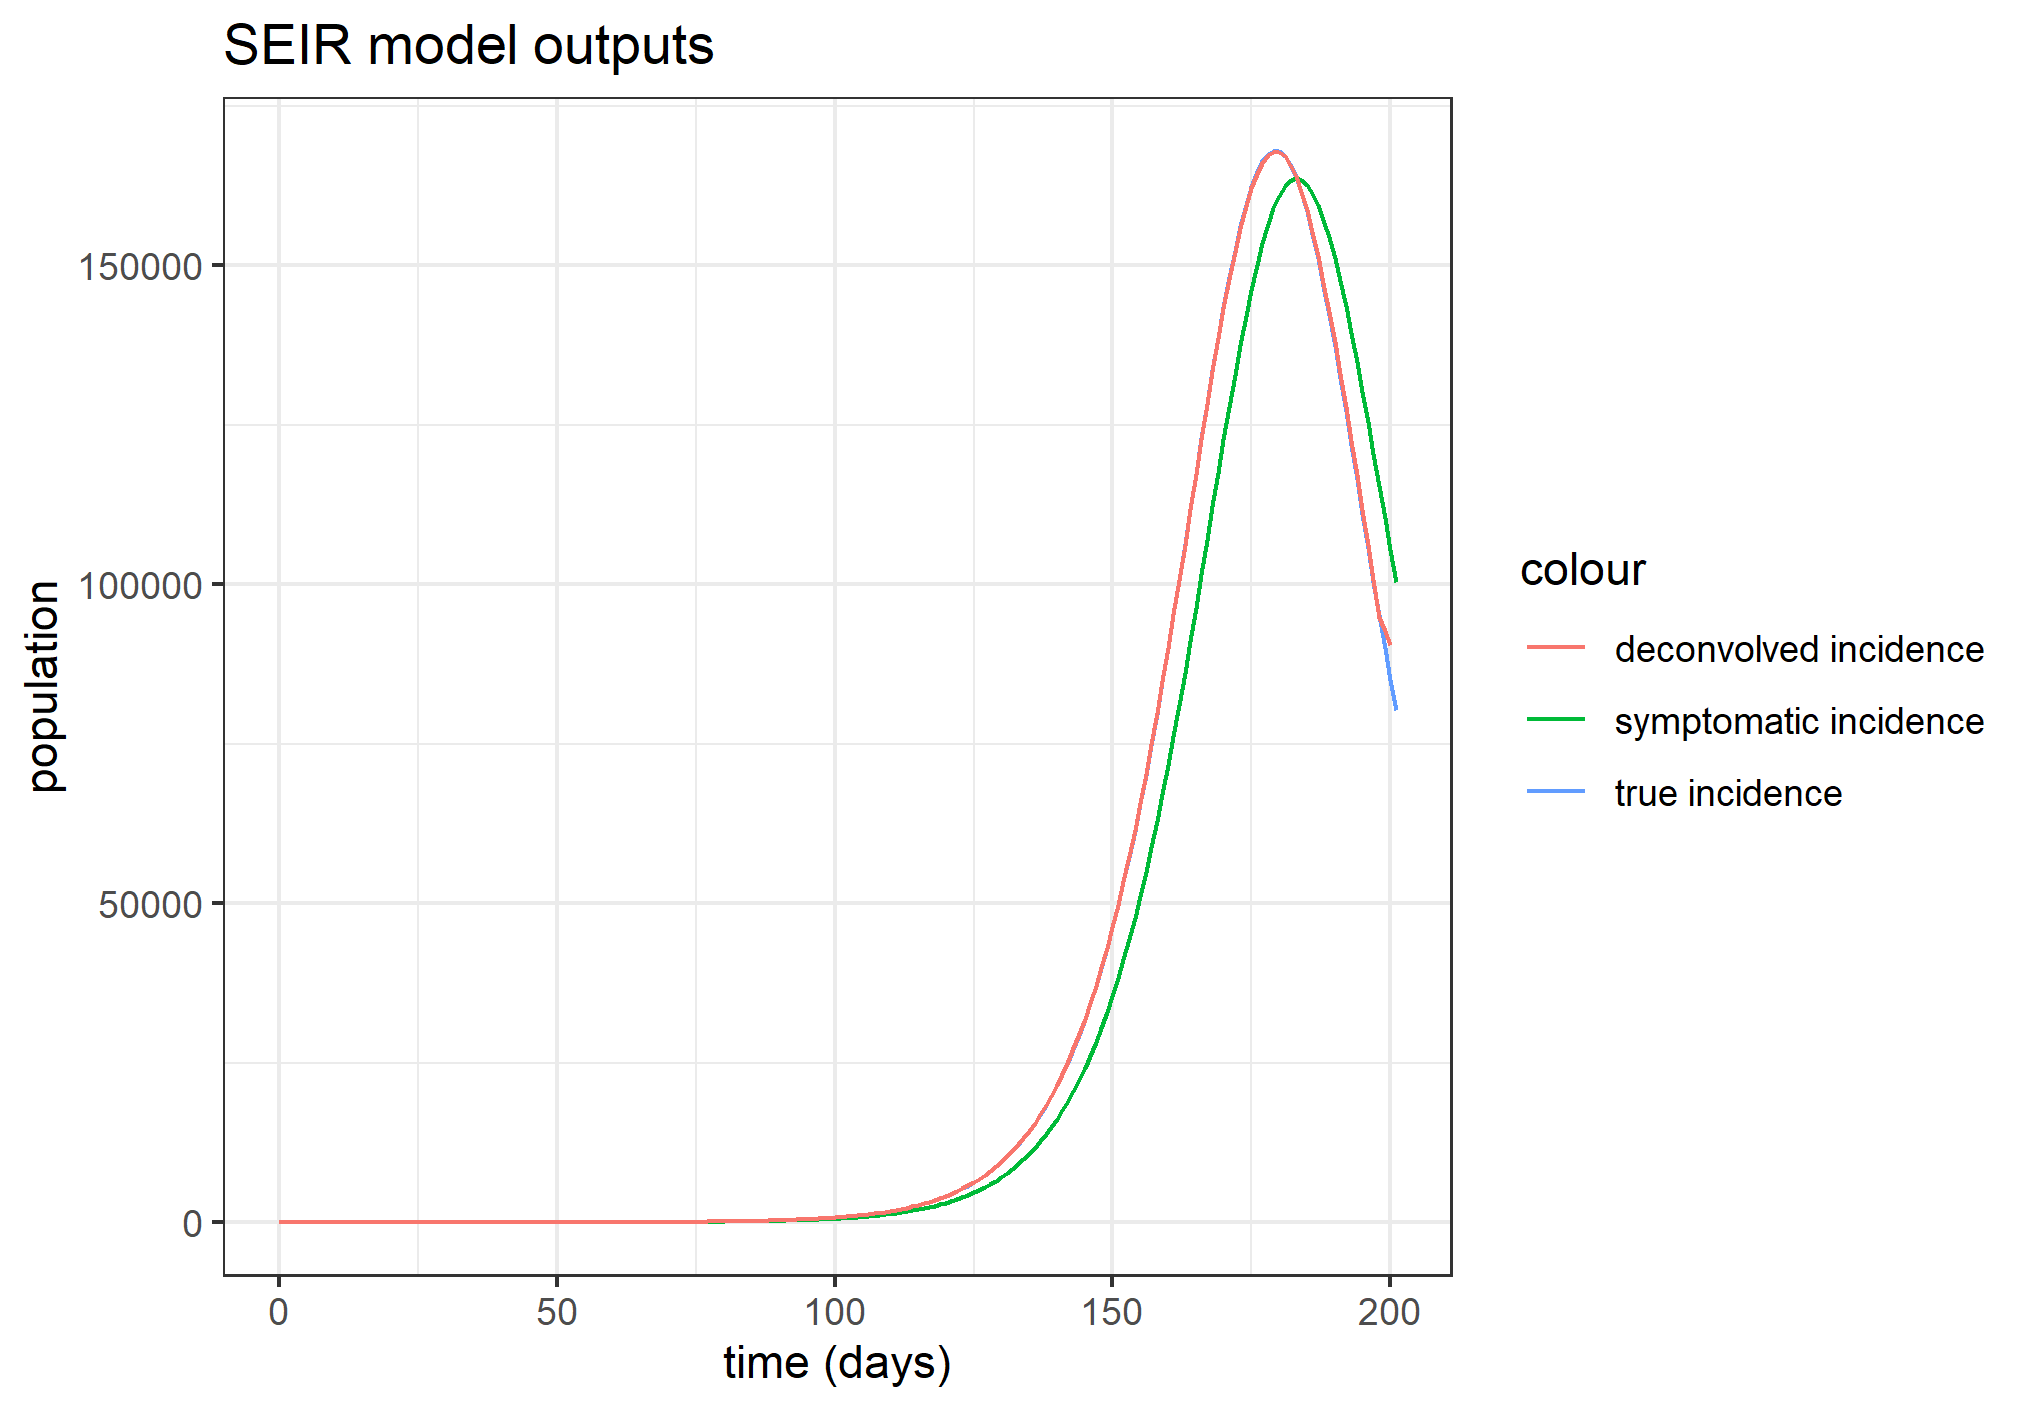
\includegraphics[scale=0.7]{figures/incidence.png}
    \caption{Deconvolved incidence, true incidence, and symptom onset curves}
    \label{fig:my_label}
\end{figure}

\begin{figure}[h!]
    \centering
    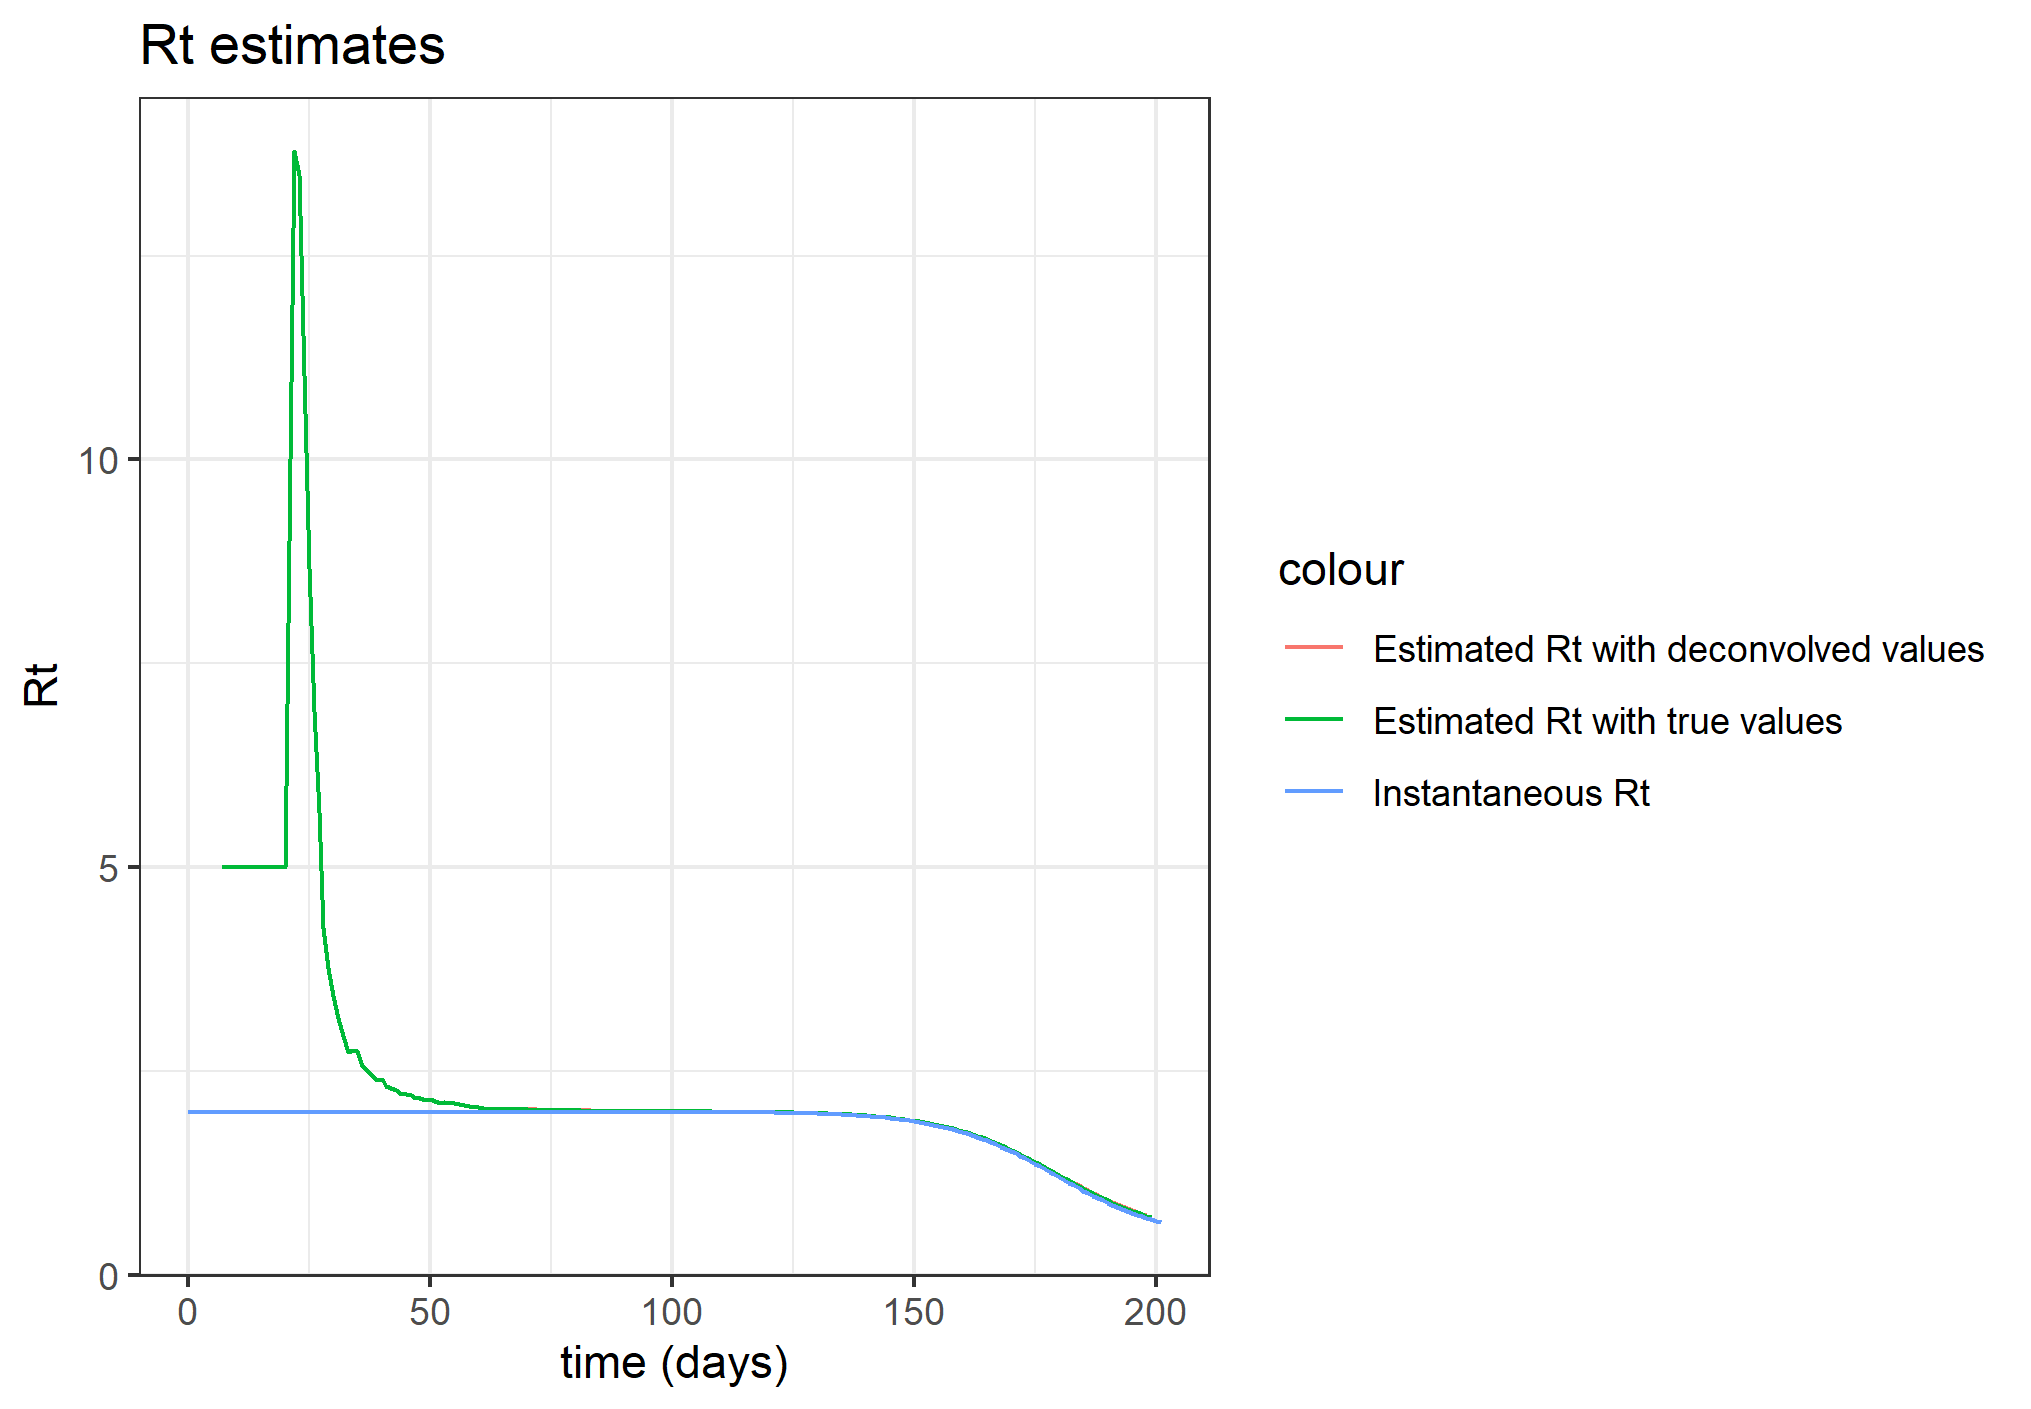
\includegraphics[scale=0.7]{figures/rt_cori_deconvolved.png}
    \caption{Instantaneous R(t) estimated with the method of Cori.}
    \label{fig:my_label}
\end{figure}

\begin{figure}[h!]
    \centering
    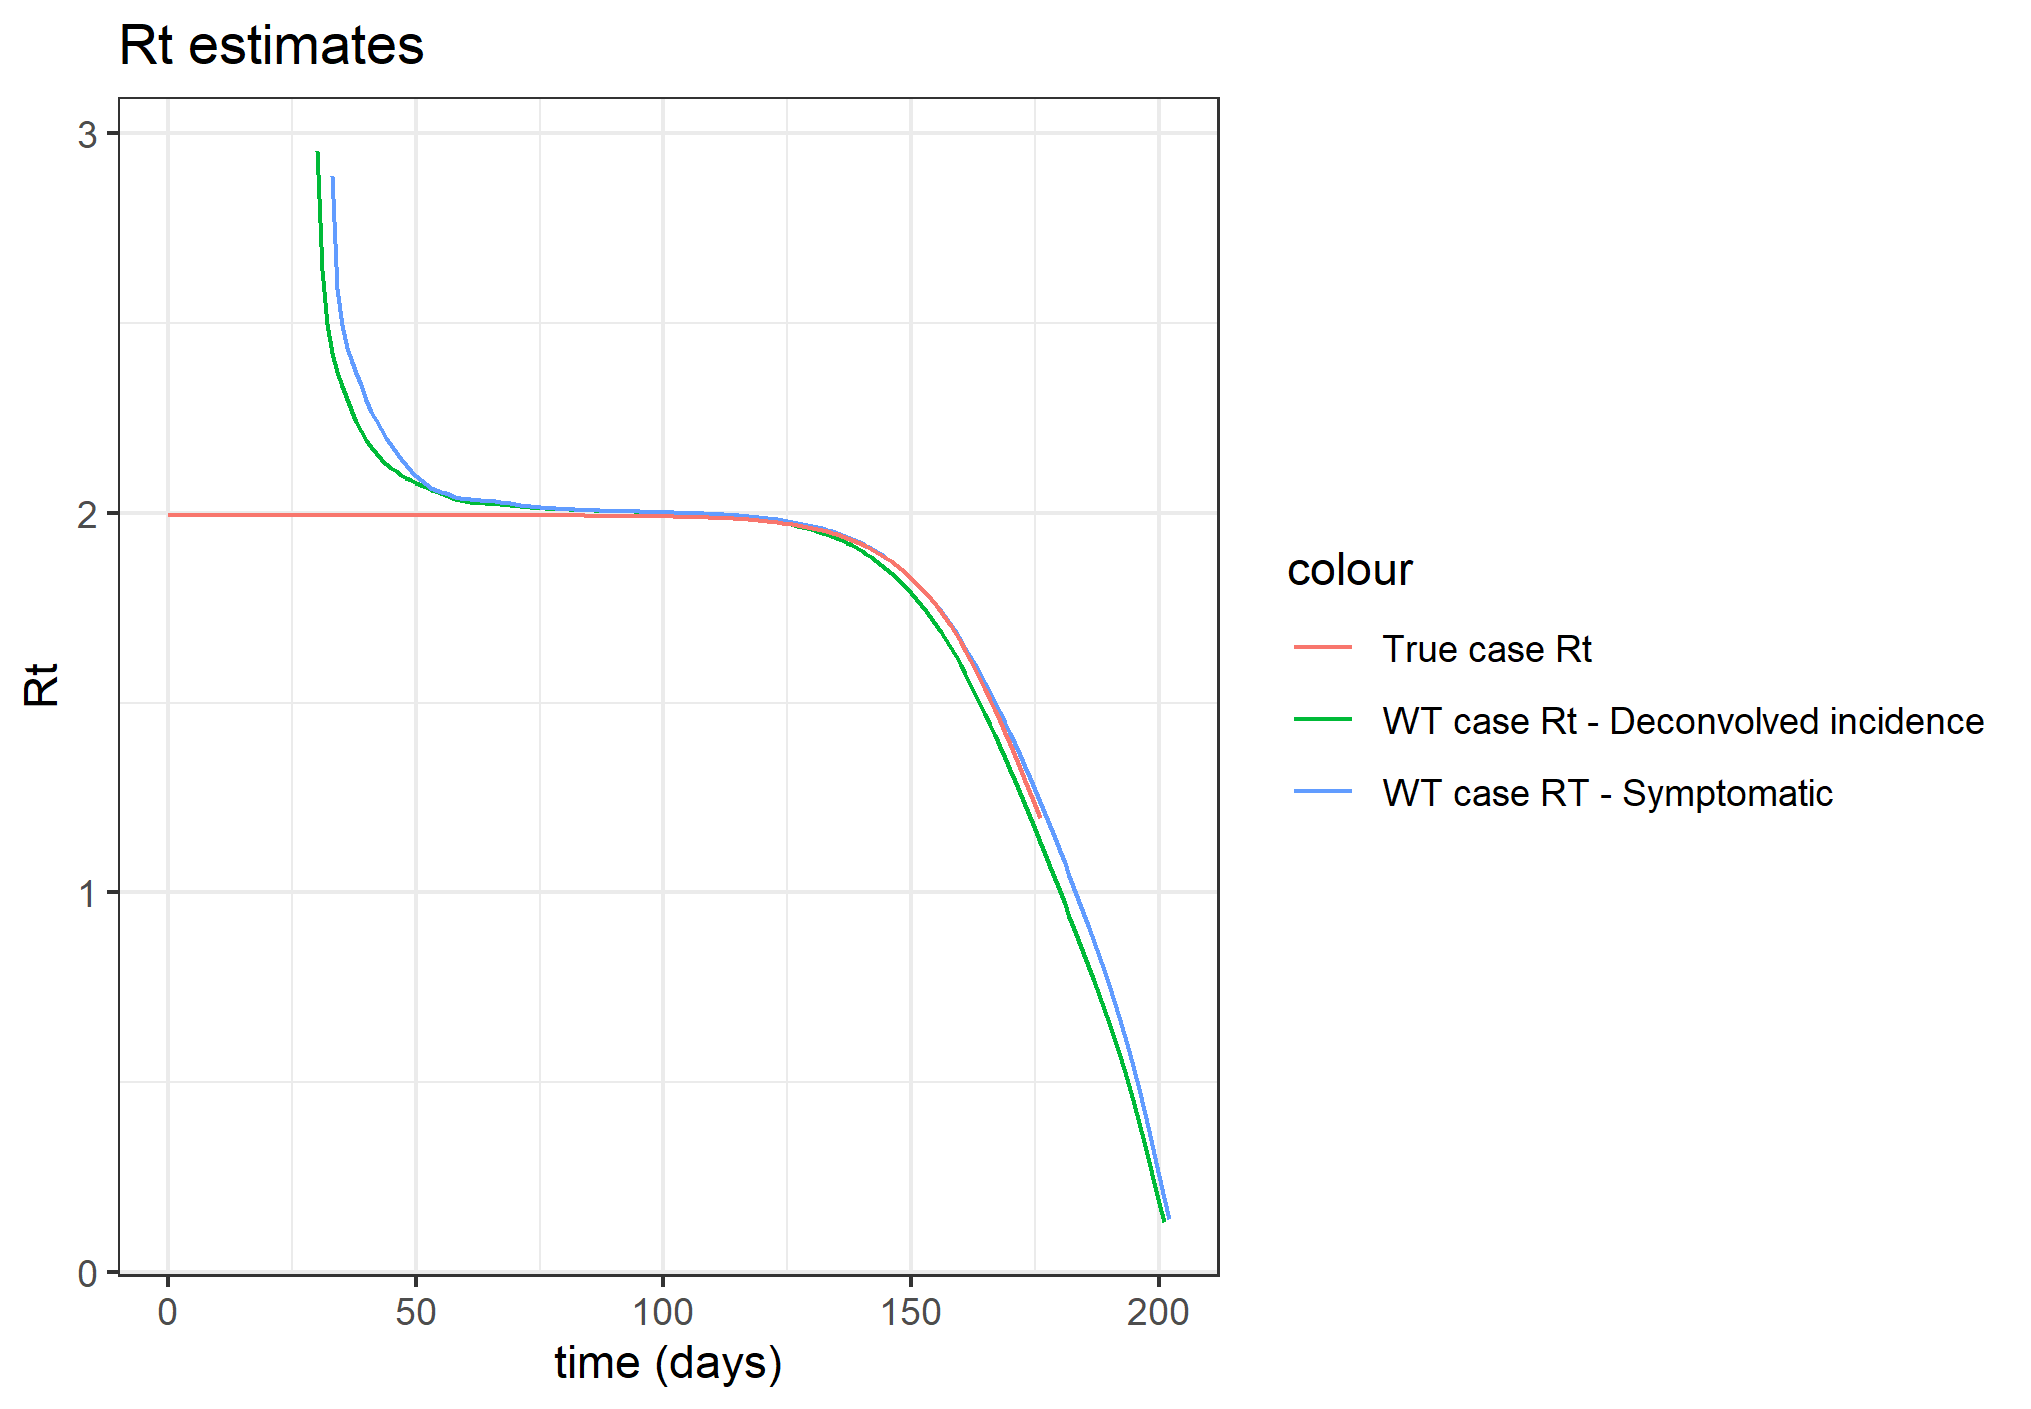
\includegraphics[scale=0.7]{figures/rt_wt.png}
    \caption{Cohort R(t) estimated with the method of Wallinga and Tenuis.}
    \label{fig:my_label}
\end{figure}


\subsection{Concerns}
\begin{itemize}
    \item The Cori estimates are no longer wrong, but the Wallinga-Tenuis ones are still slightly wrong. 
    \item I don't understand most of the math here. How was the R(t) calculated for the SEIR/other models? How does the RL deconvolution method work? How do the Cori and Wallinga estimation methods work?
\end{itemize}




\end{document}
